%%%%%%%%%%%%%%%%%%%%%%%%%%%%%%%%%%%%%%%%%
% Focus Beamer Presentation
% LaTeX Template
% Version 1.0 (8/8/18)
%
% This template has been downloaded from:
% http://www.LaTeXTemplates.com
%
% Original author:
% Pasquale Africa (https://github.com/elauksap/focus-beamertheme) with modifications by 
% Vel (vel@LaTeXTemplates.com)
%
% Template license:
% GNU GPL v3.0 License
%
% Important note:
% The bibliography/references need to be compiled with bibtex.
%
%%%%%%%%%%%%%%%%%%%%%%%%%%%%%%%%%%%%%%%%%

%----------------------------------------------------------------------------------------
%	PACKAGES AND OTHER DOCUMENT CONFIGURATIONS
%----------------------------------------------------------------------------------------

\documentclass{beamer}

\usetheme{focus} % Use the Focus theme supplied with the template
% Add option [numbering=none] to disable the footer progress bar
% Add option [numbering=fullbar] to show the footer progress bar as always full with a slide countx


\definecolor{main}{RGB}{55, 135, 177}
\definecolor{text}{RGB}{57, 100, 131}
\definecolor{background}{RGB}{255, 255, 255}

\addtobeamertemplate{block begin}{%
	\setlength{\textwidth}{0.9\textwidth}%
}{}

\addtobeamertemplate{block alerted begin}{%
	\setlength{\textwidth}{0.9\textwidth}%
}{}

\addtobeamertemplate{block example begin}{%
	\setlength{\textwidth}{0.9\textwidth}%
}{}

\setbeamercovered{transparent}

%------------------------------------------------

\usepackage{booktabs} % Required for better table rules
\usepackage{tikz}
\usepackage{xepersian}
\settextfont{Vazir}
\setsansfont{FreeSerif}
\renewcommand{\baselinestretch}{1.3}

\title{\rl{درختِ اشتاینر و فروشنده‌ی دوره‌گرد}}

\subtitle{\rl{الگوریتم‌های تقریبی}}

\author{\rl{علیرضا محمودیان}}

\titlegraphic{
\includegraphics[scale=.21]{Images/tu-logo-hckd.png}}

\institute{\rl{	دانشکده‌ی ریاضی، آمار و علومِ کامپیوتر \\ دانشگاهِ تهران}}

\date{\rl{آبان ۱۳۹۷}}


\begin{document}


\begin{frame}
	\maketitle
\end{frame}

\begin{frame}{\rl{عناوین}}
	\begin{flushright}\rl{
			$\blacksquare$ درختِ اشتاینر \\
			$\bullet~~~~~~~~~~~~~~~~~~~~$ تعریفِ مسئله \\
			$\bullet~~~~~~~~~~~~~~~~~~~~$ ناورداییِ جواب تحتِ بستارِ متریک \\
			$\bullet~~~~~~~~~~~~~~~~~~~~$ الگوریتمِ فاکتورِ ۲ \\
			$\blacksquare$ فروشنده‌ی دوره‌گرد \\
			$\bullet~~~~~~~~~~~~~~~~~~~~$ تعریفِ مسئله \\
			$\bullet~~~~~~~~~~~~~~~~~~~~$ چرا تقریب‌پذیر نیست؟ \\
			$\bullet~~~~~~~~~~~~~~~~~~~~$ الگوریتمِ فاکتورِ ۲ برای حالتِ متریک \\
			$\bullet~~~~~~~~~~~~~~~~~~~~$ بهبود به فاکتورِ ۳/۲ \\
	}\end{flushright}
\end{frame}

\section{\rl{مسئله‌ی درختِ اشتاینر}}

\begin{frame}[t]{\rl{مسئله‌ی درختِ اشتاینر}}
	\begin{flushright}\rl{
			\begin{block}{مسئله‌ی ۳.۱}
				برای گرافِ $G = <V, E>$ و زیر مجموعه‌ای از گره‌ها مانندِ $R \subseteq V$، درختی با وزنِ یالِ کمینه پیدا کنید که تمامِ $R$ را بپوشاند.\\
			$R$ را مجموعه‌ی گره‌های الزامی و $V-R$ را مجموعه‌ی گره‌های اشتاینر می‌نامیم.
			\end{block}
			\pause
			$\bullet$ می‌توان هر نمونه‌ی غیرِ متریک را با حفظِ تقریب به متریک تبدیل کرد. \\
			\pause
			$\leftarrow$ کافی است برای حالتِ متریک الگوریتمِ تقریبی ارائه دهیم.
	}\end{flushright}
\end{frame}

\begin{frame}[t]{\rl{مسئله‌ی درختِ اشتاینر: بستارِ متریک}}
	\begin{flushright}\rl{
	$\bullet$ برای گرافِ $G = <V, E>$، بستارِ متریکِ آن گرافی کامل مانندِ $G' = <V, E'>$ است که وزن هر یالِ $(u,v)$ در آن برابر با وزنِ مسیرِ با وزنِ کمینه بینِ $u$ و $v$ است. \\
	\pause
	$\bullet$ $G'$ به وضوح متریک است. \\
	\pause
	$\bullet$ هیچ یالی از $G$ دارای وزنِ بیشتری در $G'$ نیست. \\
	\pause
	$\leftarrow~~$ جواب بهینه‌ی $G'$ کرانِ پایینی برای جوابِ بهینه‌ی $G$ است.
	}\end{flushright}
\end{frame}

\begin{frame}[t]{\rl{مسئله‌ی درختِ اشتاینر: بستارِ متریک}}
	\begin{flushright}\rl{
			$\bullet$ برای هر درختِ اشتاینر مانندِ $T'$ در $G'$، می‌توان درختِ اشتاینرِ $T$ را در $G$ را طوری یافت که $|T| \leq |T'|$. \\
			\pause
			$\bullet$ کافی است هر یال را با مسیرِ متناظرِ آن جایگزین کرده و دورهای احتمالی را حذف کنیم. \\
			\pause
			در نتیجه: \\
			\begin{block}{قضیه‌ی ۳.۲}
 هر جوابِ تقریبیِ $G'$ را می‌توانیم  به جوابی با همان فاکتورِ تقریب برای $G$ تبدیل کنیم.
			\end{block}
	}\end{flushright}
\end{frame}

\begin{frame}[t]{\rl{مسئله‌ی درختِ اشتاینر: الگوریتمِ تقریبی}}
	\begin{flushright}\rl{
			\begin{exampleblock}{الگوریتمِ ۳.۱.۱}
				برای گرافِ متریکِ $G$: \\
				$~~$ درختِ کمینه‌ی پوشا روی مجموعه‌ی گره‌های الزامی را پیدا کنید.
			\end{exampleblock}
			\pause
			\begin{block}{قضیه‌ی ۳.۳}
				جوابِ الگوریتمِ ۳.۱.۱ حداکثر ۲ برابرِ جوابِ بهینه است.
			\end{block}
	}\end{flushright}
\end{frame}

\begin{frame}[t]{\rl{مسئله‌ی درختِ اشتاینر: الگوریتمِ تقریبی}}
	\begin{flushright}\rl{
			\begin{block}{لمِ میان‌بر}
				برای هر دو گره‌ی $u$ و $v$ در یک گرافِ متریک، یالِ $(u,v)$ کوتاه‌ترین مسیر بینِ $u$ و $v$ است.
			\end{block}
		\pause
		\begin{columns}[onlytextwidth]
			\column{0.5\textwidth}
			\flushleft
			% Graphic for TeX using PGF
% Title: /home/beleg/Diagram1.dia
% Creator: Dia v0.97+git
% CreationDate: Fri Feb  1 20:47:44 2019
% For: beleg
% \usepackage{tikz}
% The following commands are not supported in PSTricks at present
% We define them conditionally, so when they are implemented,
% this pgf file will use them.
\ifx\du\undefined
  \newlength{\du}
\fi
\setlength{\du}{15\unitlength}
\begin{tikzpicture}[even odd rule]
\pgftransformxscale{1.000000}
\pgftransformyscale{-1.000000}
\definecolor{dialinecolor}{rgb}{0.000000, 0.000000, 0.000000}
\pgfsetstrokecolor{dialinecolor}
\pgfsetstrokeopacity{1.000000}
\definecolor{diafillcolor}{rgb}{1.000000, 1.000000, 1.000000}
\pgfsetfillcolor{diafillcolor}
\pgfsetfillopacity{1.000000}
\pgfsetlinewidth{0.050000\du}
\pgfsetdash{}{0pt}
\pgfsetbuttcap
{
\definecolor{diafillcolor}{rgb}{0.000000, 0.000000, 0.000000}
\pgfsetfillcolor{diafillcolor}
\pgfsetfillopacity{1.000000}
% was here!!!
\definecolor{dialinecolor}{rgb}{0.000000, 0.000000, 0.000000}
\pgfsetstrokecolor{dialinecolor}
\pgfsetstrokeopacity{1.000000}
\draw (19.950000\du,12.950000\du)--(26.495789\du,12.961053\du);
}
% setfont left to latex
\definecolor{dialinecolor}{rgb}{0.000000, 0.000000, 0.000000}
\pgfsetstrokecolor{dialinecolor}
\pgfsetstrokeopacity{1.000000}
\definecolor{diafillcolor}{rgb}{0.000000, 0.000000, 0.000000}
\pgfsetfillcolor{diafillcolor}
\pgfsetfillopacity{1.000000}
\node[anchor=base west,inner sep=0pt,outer sep=0pt,color=dialinecolor] at (22.150000\du,13.804727\du){$|(u, v)|$};
% setfont left to latex
\definecolor{dialinecolor}{rgb}{0.000000, 0.000000, 0.000000}
\pgfsetstrokecolor{dialinecolor}
\pgfsetstrokeopacity{1.000000}
\definecolor{diafillcolor}{rgb}{0.000000, 0.000000, 0.000000}
\pgfsetfillcolor{diafillcolor}
\pgfsetfillopacity{1.000000}
\node[anchor=base west,inner sep=0pt,outer sep=0pt,color=dialinecolor] at (25.850000\du,13.400000\du){};
\pgfsetlinewidth{0.000000\du}
\pgfsetdash{{\pgflinewidth}{0.200000\du}}{0cm}
\pgfsetbuttcap
\pgfsetmiterjoin
\pgfsetlinewidth{0.000000\du}
\pgfsetbuttcap
\pgfsetmiterjoin
\pgfsetdash{{\pgflinewidth}{0.200000\du}}{0cm}
\definecolor{diafillcolor}{rgb}{0.000000, 0.000000, 0.000000}
\pgfsetfillcolor{diafillcolor}
\pgfsetfillopacity{1.000000}
\pgfpathellipse{\pgfpoint{19.888816\du}{12.959868\du}}{\pgfpoint{0.104079\du}{0\du}}{\pgfpoint{0\du}{0.104079\du}}
\pgfusepath{fill}
\definecolor{dialinecolor}{rgb}{0.000000, 0.000000, 0.000000}
\pgfsetstrokecolor{dialinecolor}
\pgfsetstrokeopacity{1.000000}
\pgfpathellipse{\pgfpoint{19.888816\du}{12.959868\du}}{\pgfpoint{0.104079\du}{0\du}}{\pgfpoint{0\du}{0.104079\du}}
\pgfusepath{stroke}
\pgfsetlinewidth{0.000000\du}
\pgfsetdash{{\pgflinewidth}{0.200000\du}}{0cm}
\pgfsetbuttcap
\pgfsetmiterjoin
\pgfsetlinewidth{0.000000\du}
\pgfsetbuttcap
\pgfsetmiterjoin
\pgfsetdash{{\pgflinewidth}{0.200000\du}}{0cm}
\definecolor{diafillcolor}{rgb}{0.000000, 0.000000, 0.000000}
\pgfsetfillcolor{diafillcolor}
\pgfsetfillopacity{1.000000}
\pgfpathellipse{\pgfpoint{26.574605\du}{12.958184\du}}{\pgfpoint{0.104079\du}{0\du}}{\pgfpoint{0\du}{0.104079\du}}
\pgfusepath{fill}
\definecolor{dialinecolor}{rgb}{0.000000, 0.000000, 0.000000}
\pgfsetstrokecolor{dialinecolor}
\pgfsetstrokeopacity{1.000000}
\pgfpathellipse{\pgfpoint{26.574605\du}{12.958184\du}}{\pgfpoint{0.104079\du}{0\du}}{\pgfpoint{0\du}{0.104079\du}}
\pgfusepath{stroke}
% setfont left to latex
\definecolor{dialinecolor}{rgb}{0.000000, 0.000000, 0.000000}
\pgfsetstrokecolor{dialinecolor}
\pgfsetstrokeopacity{1.000000}
\definecolor{diafillcolor}{rgb}{0.000000, 0.000000, 0.000000}
\pgfsetfillcolor{diafillcolor}
\pgfsetfillopacity{1.000000}
\node[anchor=base west,inner sep=0pt,outer sep=0pt,color=dialinecolor] at (19.337895\du,13.121053\du){$u$};
% setfont left to latex
\definecolor{dialinecolor}{rgb}{0.000000, 0.000000, 0.000000}
\pgfsetstrokecolor{dialinecolor}
\pgfsetstrokeopacity{1.000000}
\definecolor{diafillcolor}{rgb}{0.000000, 0.000000, 0.000000}
\pgfsetfillcolor{diafillcolor}
\pgfsetfillopacity{1.000000}
\node[anchor=base west,inner sep=0pt,outer sep=0pt,color=dialinecolor] at (26.740000\du,13.171579\du){$v$};
\pgfsetlinewidth{0.050000\du}
\pgfsetdash{}{0pt}
\pgfsetbuttcap
{
\definecolor{diafillcolor}{rgb}{0.000000, 0.000000, 0.000000}
\pgfsetfillcolor{diafillcolor}
\pgfsetfillopacity{1.000000}
% was here!!!
\definecolor{dialinecolor}{rgb}{0.000000, 0.000000, 0.000000}
\pgfsetstrokecolor{dialinecolor}
\pgfsetstrokeopacity{1.000000}
\draw (19.936133\du,12.866942\du)--(20.720622\du,11.326274\du);
}
\pgfsetlinewidth{0.000000\du}
\pgfsetdash{{\pgflinewidth}{0.200000\du}}{0cm}
\pgfsetbuttcap
\pgfsetmiterjoin
\pgfsetlinewidth{0.000000\du}
\pgfsetbuttcap
\pgfsetmiterjoin
\pgfsetdash{{\pgflinewidth}{0.200000\du}}{0cm}
\definecolor{diafillcolor}{rgb}{0.000000, 0.000000, 0.000000}
\pgfsetfillcolor{diafillcolor}
\pgfsetfillopacity{1.000000}
\pgfpathellipse{\pgfpoint{20.646064\du}{11.475608\du}}{\pgfpoint{0.104079\du}{0\du}}{\pgfpoint{0\du}{0.104079\du}}
\pgfusepath{fill}
\definecolor{dialinecolor}{rgb}{0.000000, 0.000000, 0.000000}
\pgfsetstrokecolor{dialinecolor}
\pgfsetstrokeopacity{1.000000}
\pgfpathellipse{\pgfpoint{20.646064\du}{11.475608\du}}{\pgfpoint{0.104079\du}{0\du}}{\pgfpoint{0\du}{0.104079\du}}
\pgfusepath{stroke}
\pgfsetlinewidth{0.050000\du}
\pgfsetdash{}{0pt}
\pgfsetbuttcap
{
\definecolor{diafillcolor}{rgb}{0.000000, 0.000000, 0.000000}
\pgfsetfillcolor{diafillcolor}
\pgfsetfillopacity{1.000000}
% was here!!!
\definecolor{dialinecolor}{rgb}{0.000000, 0.000000, 0.000000}
\pgfsetstrokecolor{dialinecolor}
\pgfsetstrokeopacity{1.000000}
\draw (26.525422\du,12.866885\du)--(25.615290\du,11.177410\du);
}
\pgfsetlinewidth{0.000000\du}
\pgfsetdash{{\pgflinewidth}{0.200000\du}}{0cm}
\pgfsetbuttcap
\pgfsetmiterjoin
\pgfsetlinewidth{0.000000\du}
\pgfsetbuttcap
\pgfsetmiterjoin
\pgfsetdash{{\pgflinewidth}{0.200000\du}}{0cm}
\definecolor{diafillcolor}{rgb}{0.000000, 0.000000, 0.000000}
\pgfsetfillcolor{diafillcolor}
\pgfsetfillopacity{1.000000}
\pgfpathellipse{\pgfpoint{25.707460\du}{11.380335\du}}{\pgfpoint{0.104079\du}{0\du}}{\pgfpoint{0\du}{0.104079\du}}
\pgfusepath{fill}
\definecolor{dialinecolor}{rgb}{0.000000, 0.000000, 0.000000}
\pgfsetstrokecolor{dialinecolor}
\pgfsetstrokeopacity{1.000000}
\pgfpathellipse{\pgfpoint{25.707460\du}{11.380335\du}}{\pgfpoint{0.104079\du}{0\du}}{\pgfpoint{0\du}{0.104079\du}}
\pgfusepath{stroke}
\pgfsetlinewidth{0.050000\du}
\pgfsetdash{{0.400000\du}{0.400000\du}}{0\du}
\pgfsetbuttcap
\definecolor{dialinecolor}{rgb}{0.000000, 0.000000, 0.000000}
\pgfsetstrokecolor{dialinecolor}
\pgfsetstrokeopacity{1.000000}
\pgfpathmoveto{\pgfpoint{25.719387\du}{11.335827\du}}
\pgfpatharc{325}{214}{3.065265\du and 3.065265\du}
\pgfusepath{stroke}
% setfont left to latex
\definecolor{dialinecolor}{rgb}{0.000000, 0.000000, 0.000000}
\pgfsetstrokecolor{dialinecolor}
\pgfsetstrokeopacity{1.000000}
\definecolor{diafillcolor}{rgb}{0.000000, 0.000000, 0.000000}
\pgfsetfillcolor{diafillcolor}
\pgfsetfillopacity{1.000000}
\node[anchor=base west,inner sep=0pt,outer sep=0pt,color=dialinecolor] at (22.757090\du,10.757611\du){$|p|$};
\end{tikzpicture}

			\column{0.5\textwidth}
			\flushright
			برای هر مسیر بینِ $u$ و $v$ مانندِ $p$،
			\[ |p| \leq |(u,v)| \]
		\end{columns}
	}\end{flushright}
\end{frame}

\begin{frame}[t]{\rl{مسئله‌ی درختِ اشتاینر: الگوریتمِ تقریبی}}
	\begin{flushright}\rl{
			\begin{block}{قضیه‌ی ۳.۳}
				جوابِ الگوریتمِ ۳.۱.۱ جوابی قابلِ قبول و حداکثر ۲ برابرِ جوابِ بهینه است.
			\end{block}
			\pause
			$\blacksquare$ فرض کنید $T$ جوابِ الگوریتم و $OPT$ جوابِ بهینه باشد. \\
			\pause
			$\bullet~~$ $T$ درختی پوشا روی $R$ و در نتیجه قابلِ قبول است. \\
			\pause
			$\bullet~~$ یال‌های $OPT$ را دوبل کنید و پیمایشِ اویلریِ آن را $C$ بنامید. $|C| = 2 . |OPT| \leftarrow $ \\
			\pause
			$\bullet~~$ $C$ را با میان‌بر زدن و حذف گره‌های اشتاینر و گره‌های الزامیِ تکراری به یک دورِ همیلتونی مانندِ $H$ تبدیل کنید.\\
			\pause
			$\bullet~~$ لمِ میان‌بر $|H| \leq |C| \leftarrow$
	}\end{flushright}
\end{frame}

\begin{frame}[t]{\rl{مسئله‌ی درختِ اشتاینر: الگوریتمِ تقریبی}}
	\begin{flushright}\rl{
			\begin{block}{قضیه‌ی ۳.۳}
				جوابِ الگوریتمِ ۳.۱.۱ جوابی قابلِ قبول و حداکثر ۲ برابرِ جوابِ بهینه است.
			\end{block}
			\pause
			$\bullet~~$ با حذفِ یک یال از دورِ $H$، یک درختِ پوشا روی $R$ خواهیم داشت، که آن را $T'$ می‌نامیم. $|T'| \leq |H| \leftarrow$ \\
			\pause
			$\bullet~~$ اما $T$ کم‌وزن‌ترین درختِ پوشای $R$ است $|T| \leq |T'| \leftarrow$ \\
			\pause
			\[ |T| \leq |T'| \leq |H| \leq |C| = 2.|OPT| \]
			\[ |T| \leq 2.|OPT| \]
	}\end{flushright}
\end{frame}


\begin{frame}[t]{\rl{مسئله‌ی درختِ اشتاینر: مثال از بدترین حالت}}
	\begin{flushright}\rl{
			مثالِ ۳.۴
		\begin{columns}[onlytextwidth]
			\column{0.5\textwidth}
			\flushleft
			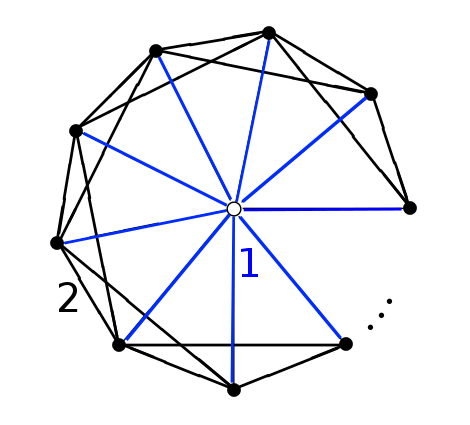
\includegraphics[width=\linewidth]{Images/steiner-tree-tight-example.png}
			\column{0.5\textwidth}
			\flushright
			\[ |T| = 2(n-1) \]
			\[ |OPT| = n \]
		\end{columns}
	}\end{flushright}
\end{frame}


\section{\rl{مسئله‌ی فروشنده‌ی دوره‌گرد}}

\begin{frame}{\rl{مسئله‌ی فروشنده‌ی دوره‌گرد}}
    \begin{flushright}\rl{
    	\begin{block}{مسئله‌ی ۳.۵}
             پیداکردنِ دورِ همیلتونی با وزنِ کمینه
    	\end{block}
	    \pause
        $\bullet$ در حالتِ کلی تقریب‌پذیر نیست. \\
        \pause
        $\bullet$ تابعِ وزنِ متریک $~\leftarrow~$ \\
        $\bullet~~~~~~~~~~~~~~~~~~~~~~~~~~~~~~~~~~~~~$ الگوریتم ۱: فاکتورِ ۲ \\
        \pause
        $\bullet~~~~~~~~~~~~~~~~~~~~~~~~~~~~~~~~~~~~~$ الگوریتم ۲: بهبود به فاکتورِ ۳/۲ \\
    }\end{flushright}
\end{frame}

\begin{frame}[t]{\rl{مسئله‌ی فروشنده‌ی دوره‌گرد: عدمِ تقریب‌پذیری}}
	\begin{flushright}\rl{
			\begin{block}{قضیه‌ی ۳.۶}
				برای هر $\alpha(n)$-تقریب از TSP مانندِ $\alpha(n)TSP$، داریم: $HAMPATH \leq_{PTIME} \alpha(n)TSP$
			\end{block}
			\pause
			$\blacksquare$ فرض کنیم الگوریتمِ تقریبی با فاکتورِ $\alpha(n)$ برای $TSP$ وجود دارد. \\
			\pause
			$\bullet~~$ برای یک نمونه‌ی مسئله‌ی دورِ همیلتونی مانندِ $G$:\\
			$\bullet~~~~$ به تمامِ یال‌های $G$ وزنِ ۱ بدهید. \\
			\pause
			$\bullet~~~~$ بینِ هر دو گره‌ی بدونِ یال، یالی با وزنِ $n.\alpha(n)$ اضافه کنید.\\
			\pause
			$\bullet~~$ $\alpha(n)TSP$ را روی گرافِ حاصل اجرا کنید.
	}\end{flushright}
\end{frame}

\begin{frame}[t]{\rl{مسئله‌ی فروشنده‌ی دوره‌گرد: عدمِ تقریب‌پذیری}}
	\begin{flushright}\rl{
			\begin{block}{قضیه‌ی ۳.۶}
				برای هر $\alpha(n)$-تقریب از TSP مانندِ $\alpha(n)TSP$، داریم: $HAMPATH \leq_{PTIME} \alpha(n)TSP$
			\end{block}
			$\bullet~~$ اگر $\leftarrow |\alpha(n)TSP| = n$ $G$ دورِ همیلتونی دارد. \\
			\pause
			$\bullet~~$ اگر $\leftarrow |\alpha(n)TSP| > n.\alpha(n)$ $G$ دورِ همیلتونی ندارد. \\
			\pause
			\[ HAMPATH \leq_{PTIME} \alpha(n)TSP \]
			\pause
			$\Leftarrow$ با فرضِ $P \neq NP$، $TSP$ در حالتِ کلی تقریب‌پذیر نیست.
	}\end{flushright}
\end{frame}

\begin{frame}[t]{\rl{مسئله‌ی فروشنده‌ی دوره‌گرد: الگوریتمِ با فاکتورِ ۲}}
	\begin{flushright}\rl{
			\begin{exampleblock}{الگوریتمِ ۳.۷}
				برای گرافِ متریکِ $G$: \\
				۱. درختِ پوشای کمینه‌ی $G$ را پیدا کنید $\leftarrow$ $T$ \\
				۲. یال‌های $T$ را دوبل کنید $\leftarrow$ $G'$ \\
				۳. یک پیمایشِ اویلری از $G'$ پیدا کنید $\leftarrow$ $\mathcal{T}$ \\
				۴. دنباله‌ای از گره‌ها به ترتیبِ اولین حضور در $\mathcal{T}$ تشکیل داده و اولین گره را در انتها تکرار کنید $\leftarrow$ $H$
			\end{exampleblock}
	}\end{flushright}
\end{frame}

\begin{frame}[t]{\rl{مسئله‌ی فروشنده‌ی دوره‌گرد: الگوریتمِ با فاکتورِ ۲}}
	\begin{flushright}\rl{
			\begin{block}{قضیه‌ی ۳.۸}
				الگوریتمِ ۳.۷ یک الگوریتمِ تقریبی با فاکتورِ ۲ برای $TSP$ متریک است.
			\end{block}
		\pause
		$\bullet$ با حذفِ یک یال از هر دورِ همیلتونی یک درختِ پوشا خواهیم داشت $\leftarrow$ درختِ پوشای کمینه کرانِ پایینی برای جوابِ $TSP$ است. $\leftarrow$ $|T| \leq |OPT|$ \\
		\pause
		$\bullet$ هر یالِ $T$ دو بار در $\mathcal{T}$ تکرار می‌شود $\leftarrow$ 
		$|\mathcal{T}| = 2.|T|$ \\
		\pause
		$\bullet$ گامِ ۴ گره‌های تکراری را حذف می‌کند، از لمِ میان‌بر $\leftarrow$ $|H| \leq |\mathcal{T}|$ \\
		\pause
		$\bullet$ همچنین $H$ یک دورِ همیلتونی از $G$ است.
	}\end{flushright}
\end{frame}

\begin{frame}[t]{\rl{مسئله‌ی فروشنده‌ی دوره‌گرد: الگوریتمِ با فاکتورِ ۲}}
	\begin{flushright}\rl{
			\begin{block}{قضیه‌ی ۳.۸}
				الگوریتمِ ۳.۷ یک الگوریتمِ تقریبی با فاکتورِ ۲ برای $TSP$ متریک است.
			\end{block}
		\[ |H| \leq |\mathcal{T}| = 2.|T| \leq 2.|OPT| \]
		\[ |H| \leq 2.|OPT| \]
	}\end{flushright}
\end{frame}

\begin{frame}[t]{\rl{مسئله‌ی فروشنده‌ی دوره‌گرد: مثال از بدترین حالت}}
	\begin{flushright}\rl{
			مثالِِ ۳.۹
		\begin{columns}[onlytextwidth]
			\column{0.5\textwidth}
			\flushleft
			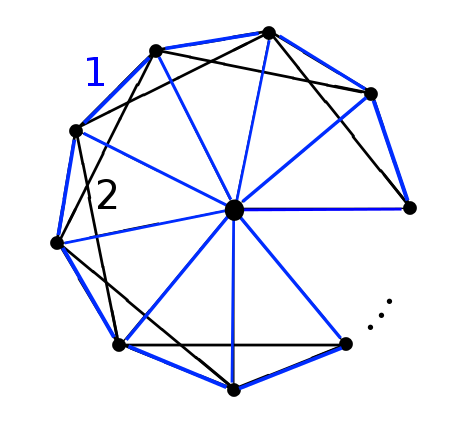
\includegraphics[width=\linewidth]{Images/tsp-2-tight-example.png}
			\column{0.5\textwidth}
			\flushright
			\[ |H| = 2(n-2) \]
			\[ |OPT| = n \]
		\end{columns}
	}\end{flushright}
\end{frame}

\begin{frame}[t]{\rl{مسئله‌ی فروشنده‌ی دوره‌گرد: الگوریتمِ با فاکتورِ ۳/۲}}
	\begin{flushright}\rl{
			دقت کنید برای پیمایش اویلری یک گراف لازم نیست یال‌ها را دوبل کنیم، کافی است درجه‌ی همه‌ی رئوس را زوج کنیم. \\
			\pause
			اضافه‌کردنِ انطباقِ کامل همین کار را می‌کند. \\
			\pause
			\begin{exampleblock}{الگوریتمِ ۳.۱۰}
				برای گرافِ متریکِ $G$: \\
				۱. درختِ پوشای کمینه‌ی $G$ را پیدا کنید $\leftarrow$ $T$ \\
				۲. روی گره‌های درجه فردِ $T$ یک انطباقِ کامل پیدا کرده و آن را به گراف اضافه کنید $\leftarrow$ $G'$ \\
				۳. یک پیمایشِ اویلری از $G'$ پیدا کنید $\leftarrow$ $\mathcal{T}$ \\
				۴. دنباله‌ای از گره‌ها به ترتیبِ اولین حضور در $\mathcal{T}$ تشکیل دهید $\leftarrow$ $H$
			\end{exampleblock}
	}\end{flushright}
\end{frame}

\begin{frame}[t]{\rl{مسئله‌ی فروشنده‌ی دوره‌گرد: الگوریتمِ با فاکتورِ ۳/۲}}
	\begin{flushright}\rl{
			\begin{block}{لمِ ۳.۱۱}
				فرض کنید برای یک گرافِ دل‌خواه، $\tau$ جوابِ بهینه‌ی مسئله‌ی $TSP$، $V'$ زیرمجموعه‌ای با اندازه‌ی زوج از گره‌ها و $M$ انطباقِ کاملِ کمینه روی $V'$ باشد. آن‌گاه $|M| \leq |\tau|/2$.
			\end{block}
		\pause
		$\bullet$ با حذف گره‌های خارج از $V'$، $\tau$ را میان‌بر زده و آن را $\tau'$ بنامید $\leftarrow$ $|\tau'| \leq |\tau|$ \\
		\pause
		$\bullet$ چون $\tau'$ دورِ ساده‌ای با طولِ زوج است، می‌توان آن را به  ۲ انطباقِ کامل با $|V'|/2$ یال افراز کرد. \\
		\pause
		$\bullet$ از بینِ ۲ انطباقِ کاملِ$\tau'$  آن‌که وزنِ کم‌تر دارد را $M'$ بنامید $\leftarrow$ $|M'| \leq 2.|\tau'|$ \\
	}\end{flushright}
\end{frame}


\begin{frame}[t]{\rl{مسئله‌ی فروشنده‌ی دوره‌گرد: الگوریتمِ با فاکتورِ ۳/۲}}
	\begin{flushright}\rl{
			\begin{block}{لمِ ۳.۱۱}
				فرض کنید برای یک گرافِ دل‌خواه، $\tau$ جوابِ بهینه‌ی مسئله‌ی $TSP$، $V'$ زیرمجموعه‌ای با اندازه‌ی زوج از گره‌ها و $M$ انطباقِ کاملِ کمینه روی $V'$ باشد. آن‌گاه $|M| \leq |\tau|/2$.
			\end{block}
			$\bullet$ از طرفی $M$ انطباقِ کامل با وزنِ کمینه است $\leftarrow$ $|M| \leq |M'|$ \\
			\pause
			\[ |M| \leq |M'| \leq 2.|\tau'| \leq 2.|\tau| \]
			\[ |M| \leq 2.|\tau| \]
	}\end{flushright}
\end{frame}

\begin{frame}[t]{\rl{مسئله‌ی فروشنده‌ی دوره‌گرد: الگوریتمِ با فاکتورِ ۳/۲}}
	\begin{flushright}\rl{
			\begin{block}{قضیه‌ی ۳.۱۲}
				الگوریتمِ ۳.۱۰ یک الگوریتمِ تقریبی با فاکتورِ ۳/۲ برای $TSP$ متریک است.
			\end{block}
			\pause
			$\bullet$ بر خلافِ الگوریتمِ قبل، یال‌های درختِ پوشای کمینه را دوبل نمی‌کنیم.$\leftarrow$ $|\mathcal{T}| \leq |T| + |M|$. \\
			\pause
			$\bullet$ چون تعدادِ گره‌های دارای درجه‌ی فرد، زوج است، می‌توانیم لمِ ۳.۱۱ را اعمال کنیم $\leftarrow$ $\mathcal{T} \leq |T| + |OPT|/2$ \\
			\pause
			\[ |H| \leq |\mathcal{T}| = |T| + |M| \leq |OPT| + |OPT|/2 \]
			\[ |H| \leq 3/2.|OPT| \]
	}\end{flushright}
\end{frame}

\begin{frame}[t]{\rl{مسئله‌ی فروشنده‌ی دوره‌گرد: مثال از بدترین حالت}}
	\begin{flushright}\rl{
			مثالِِ ۳.۱۳
			\begin{columns}[onlytextwidth]
				\column{0.7\textwidth}
				\flushleft
				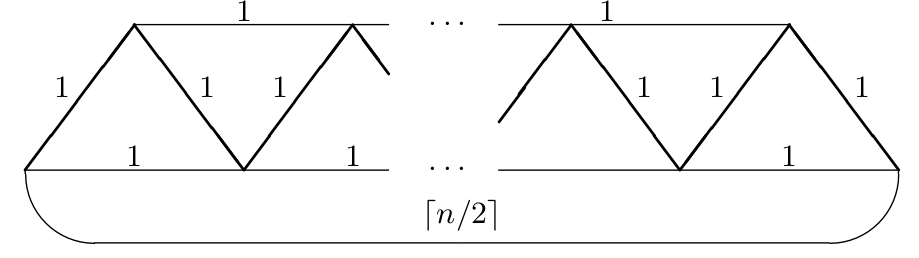
\includegraphics[width=\linewidth]{Images/tsp-3-2-tight-example.png}
				\column{0.3\textwidth}
				\flushright
				\[ |H| = n - 1 + \lceil n/2 \rceil \]
				\[ |OPT| = n \]
			\end{columns}
	}\end{flushright}
\end{frame}

%\begin{frame}[noframenumbering]{\rl{نوآوری‌های اخیر}}
%	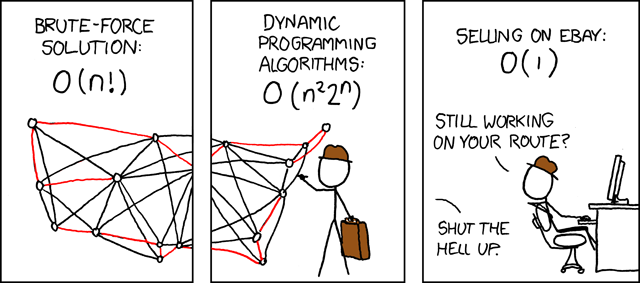
\includegraphics[width=\linewidth]{Images/travelling_salesman_problem.png}
%\end{frame}

\end{document}
